\chapter{Validation in liquid jet in crossflow}
	\label{ch6:jicf_lgs_simulations}


Describe here all our results from the lagrangian simulations:

\begin{itemize}

	\item Effects of applying full workflow: w/wo ALM, w/wo secondary atomization ...
	
	\item Mesh convergence study: specify it
	
	\item Validation with experiments
	
	\item Mass conservation issues: lagrangian tracking, etc. 
	

\end{itemize}

\section{Introduction}

\section{Models sensitivity}

ALSO: effect of one and two-way coupling !! Ver articulos 2010, 2011 Li 

\subsection{Effect of injection conditions}

\subsection{Effect of secondary atomization model}

\subsection{Effect of dense core blockage effect model}

\section{Results}

\subsection{Mesh convergence study}

\subsection{Validation with experiments (quantitative/qualitative)}

\subsection{Trajectories}

In order to illustrate the lagrangian trajectories and the continuity with respect to the resolved jets, a volume fraction field can be defined in the lagrangian simulations:

\begin{equation}
\alpha_l \left( \textbf{x}, t \right) = \frac{V_l \left( \textbf{x}, t \right)}{V_{el}}
\end{equation}

where $V_{el}$ is the volume of the element in the eulerian mesh grid. Therefore, the volume fraction is a magnitude defined in the main eulerian grid. Since the dispersed phase is not directly represented in this grid but by lagrangian particles, $V_l \left( \textbf{x}, t \right)$ is calculated by interpolating the volume of the particles located within each element at each iteration.

\subsection{Frequential analysis}

Several probes have been located in the outer part of the jet to see the spectra. See Figures \ref{fig:probes_dx10m} and \ref{fig:probes_dx20m} for volume fraction probes, and Figure \ref{fig:probes_U_planey0} for determining velocity spectra at plane y = 0. These are available at pilotage 30-04-2021.

Para velocidades: OJITO con la probe 18 !

\begin{figure}[h!]
	\centering
	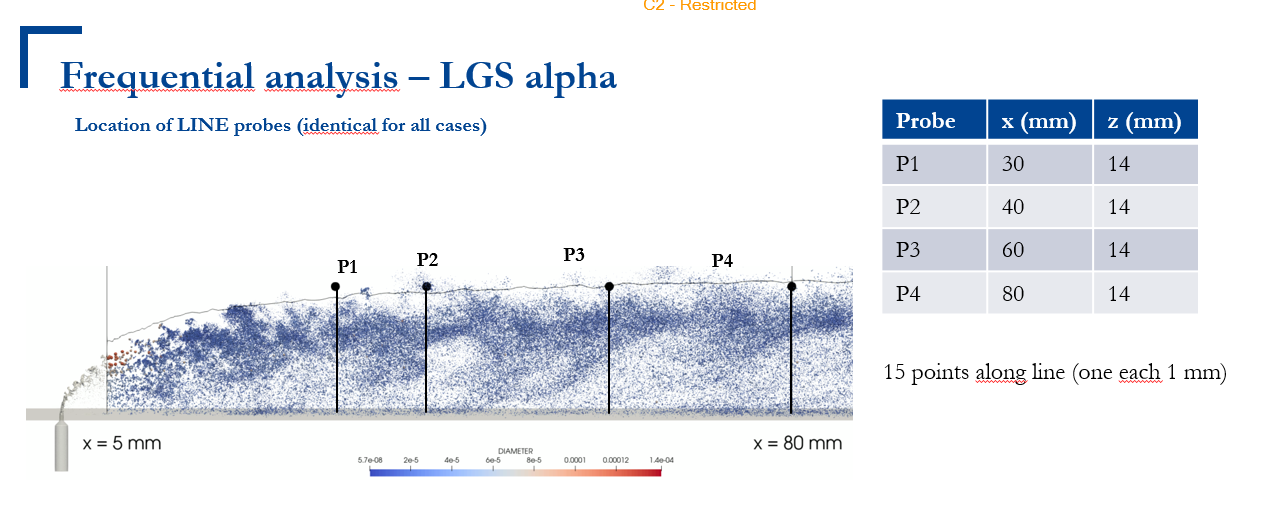
\includegraphics[scale=0.7]{./part2_developments/figures_ch6_lagrangian_JICF/probes_vol_frac}
	\caption{Probes for $\alpha$ frequential analysis for volume fraction}
	\label{fig:probes_dx10m}
\end{figure}


\begin{figure}[h!]
	\centering
	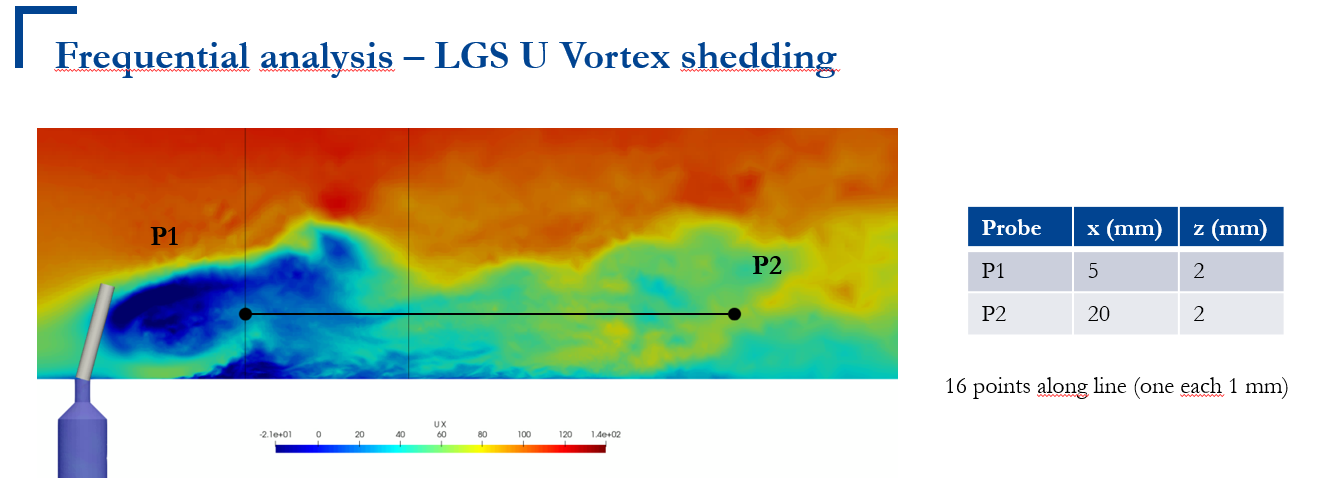
\includegraphics[scale=0.7]{./part2_developments/figures_ch6_lagrangian_JICF/probes_U_planey0}
	\caption{Probes for $U$ study}
	\label{fig:probes_U_planey0}
\end{figure}



\section{Conclusions}